\documentclass{article}
\usepackage{graphicx}
\usepackage{amssymb}
\usepackage{subfigure}
\usepackage{geometry}
\usepackage{bm}
\usepackage{fancyhdr}
\usepackage{minted}
\geometry{a4paper,left=3cm,right=3cm,top=3cm,bottom=3cm}
\usepackage{amsmath}
\pagestyle{plain}
\title{CMSE890 Homework\#3}
\author{Haiyang Yu}
\begin{document}
\maketitle
\subsection*{1.}
\subsubsection*{(1)}
$f(\bm{x})=||\bm{x}||_{1}$, so
$$
f^{*}(\bm{y})=\left\{
\begin{aligned}
&+\infty,&\ \ \ ||\bm{y}||_{\infty}>1\\
&0,&\ \ \ ||\bm{y}||_{\infty}\leq1
\end{aligned}
\right.
$$
Define
$$
h(\bm{y})=f^{*}(\bm{y})+d(\bm{y})=\left\{
\begin{aligned}
&\mu\sum_{i=1}^{n}(1-\sqrt{1-y_{i}^{2}}),&\ \ \ ||\bm{y}||_{\infty}\leq1\\
&+\infty,&\ \ \ ||\bm{y}||_{\infty}>1
\end{aligned}
\right.
$$
Thus,
\begin{align*}
h^{*}(\bm{x})&=\sup_{\bm{y}}\bm{x}^{\mathrm{T}}\bm{y}-h(\bm{y})\\
&=\sup_{||\bm{y}||_{\infty}\leq 1}\bm{x}^{\mathrm{T}}\bm{y}-\mu\sum_{i=1}^{n}(1-\sqrt{1-y_{i}^{2}})\\
&=\sum_{i=1}^{n}\sup_{|y_{i}|\leq 1}\left\{x_{i}y_{i}-\mu(1-\sqrt{1-y_{i}^{2}})\right\}\\
&=\sum_{i=1}^{n}\left[x_{i}y_{i}-\mu(1-\sqrt{1-y_{i}^{2}})\right]_{y_{i}={x_{i}}/{\sqrt{\mu^{2}+x_{i}^{2}}}}\\
&=\sum_{i=1}^{n}\sqrt{x_{i}^{2}+\mu^{2}}-\mu
\end{align*}
\subsubsection*{(2)}
$f(\bm{x})=\max_{i}x_{i}$, so
$$
f^{*}(\bm{y})=\left\{
\begin{aligned}
0,&\ \ \ \mathrm{if}\ \sum_{i=1}^{n}y_{i}=1,\ \mathrm{and}\ y_{i}\geq0\ \mathrm{for\ all\ }i\\
+\infty,&\ \ \ \mathrm{else}
\end{aligned}
\right.
$$
Define
$$
h(\bm{y})=f^{*}(\bm{y})+d(\bm{y})=\left\{
\begin{aligned}
&\mu\sum_{i=1}^{n}\left(y_{i}\log{y_{i}}+\log{n}\right),&&\mathrm{if}\ \sum_{i=1}^{n}y_{i}=1,\ \mathrm{and}\ y_{i}\geq0\ \mathrm{for\ all\ }i\\
&+\infty,&&\mathrm{else}
\end{aligned}
\right.
$$
Thus,
\begin{align*}
h^{*}(\bm{x})&=\sup_{\bm{y}}\bm{x}^{\mathrm{T}}\bm{y}-h(\bm{y})\\
&=\sup_{\substack{\sum_{i=1}^{n}y_{i}=1\\ y_{i}\geq0}}\left\{\bm{x}^{\mathrm{T}}\bm{y}-\mu\sum_{i=1}^{n}\left(y_{i}\log{y_{i}}+\log{n}\right)\right\}\\
&=\left.\sum_{i=1}^{n}x_{i}y_{i}-\mu y_{i}\log{y_{i}-\mu\log{n}}\right|_{y_{i}=\frac{\mathrm{e}^{\frac{x_{i}}{\mu}-1}}{\sum_{i=1}^{n}\mathrm{e}^{\frac{x_{i}}{\mu}-1}}}\\
&=\mu+\mu\log{\left(\sum_{i=1}^{n}\mathrm{e}^{\frac{x_{i}}{\mu}-1}\right)}-\mu n \log{n}
\end{align*}
\subsection*{2.}
$f(X)=-\log{\det{X}}$.Suppose $X=P^{\mathrm{T}}\Lambda P$, where $P$ is orthogonal matrix and $\Lambda=\mathrm{diag}(\lambda_{1},\lambda_{2},\cdots,\lambda_{n})$ is a diagonal matrix with positive eigenvalues.
$U$ has positive eigenvalues $u_{i}$.
\begin{align*}
\mathrm{prox}_{f}(X)&=\mathop{\arg\min}_{U}-\log{\det{U}}+\frac{1}{2}||U-X||^{2}_{F}\\
&=\mathop{\arg\min}_{U}-\log{\det{PUP^{-1}}}+\frac{1}{2}||P^{-1}(PUP^{-1}-\Lambda)P||_{F}^{2}\\
&=P^{-1}\left(\mathop{\arg\min}_{U}-\log{\det{U}}+\frac{1}{2}||U-\Lambda||_{F}^{2}\right)P\\
&=P^{-1}\left(\mathop{\arg\min}_{U}\sum_{i=1}^{n}-\log{u_{i}}+\frac{1}{2}(u_{i}-\lambda_{i})^{2}\right)P\\
&=P^{-1}\mathrm{diag(\frac{\lambda_{1}+\sqrt{\lambda_{1}^{2}+4}}{2},\frac{\lambda_{2}+\sqrt{\lambda_{2}^{2}+4}}{2},\cdots,\frac{\lambda_{n}+\sqrt{\lambda_{n}^{2}+4}}{2})}P
\end{align*}
\subsubsection*{(3)}
\begin{figure}[!h]
  \centering
  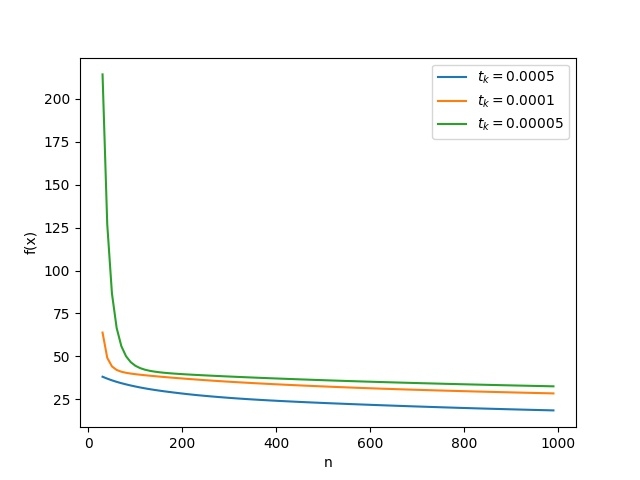
\includegraphics[width=8cm]{1.jpg}\\
\end{figure}
\begin{minted}{python}
import numpy as np
import matplotlib.pyplot as plt

def partial(x):
    tmp=A.dot(x)-b
    res=A.T.dot(tmp)
    return res

def prox(t,x):   #when h(x)=||x||_{1}
    res=np.zeros((len(x),1))
    for i in range(len(x)):
        if x[i]>t:
            res[i]=x[i]-t
        if x[i]<-t:
            res[i]=x[i]+t
    return res

def f(x):
    s1=0
    for i in range(len(x)):
        s1+=abs(x[i])
    tmp=A.dot(x)-b
    s2=np.dot(tmp.T,tmp)
    return s1+s2


np.random.seed(1000)
m=200
n=1000
A=np.random.normal(0,1,(m,n))
x_bar=np.zeros((n,1))
for i in range(20):
    k=np.random.randint(0,1000)
    x_bar[k]=np.random.normal(0,1)
b=A.dot(x_bar)

x_pre=np.zeros((n,1))
y1=[]
n1=[]
y2=[]
n2=[]
y3=[]
n3=[]
iteration=1000
for i in range(iteration):
    tk=0.0005
    x_now=prox(tk,x_pre-tk*partial(x_pre))
    x_pre=x_now
    if i%10==0 and i>20:
        y1.append(f(x_now)[0][0])
        n1.append(i)
x_pre=np.zeros((n,1))
for i in range(iteration):
    tk=0.0001
    x_now=prox(tk,x_pre-tk*partial(x_pre))
    x_pre=x_now
    if i%10==0 and i>20:
        y2.append(f(x_now)[0][0])
        n2.append(i)
x_pre=np.zeros((n,1))
for i in range(iteration):
    tk=0.00005
    x_now=prox(tk,x_pre-tk*partial(x_pre))
    x_pre=x_now
    if i%10==0 and i>20:
        y3.append(f(x_now)[0][0])
        n3.append(i)
plt.plot(n1,y1,label=r'$t_{k}=0.0005$')
plt.plot(n2,y2,label=r'$t_{k}=0.0001$')
plt.plot(n3,y3,label=r'$t_{k}=0.00005$')
plt.xlabel("n")
plt.ylabel("f(x)")
plt.legend()
plt.show()

\end{minted}
\end{document}
